\chapter{General Methodology}

\section{Problems}

There exist a number of problems when doing strength training-based fitness tracking. The first is the issue of \textit{separating exercise from non-exercise}. As with most problems in machine learning, exercise is easily discerned from non-exercise when viewed with the naked eye. This separability breaks down when viewing exercise from the perspective of the onboard sensors. Performing a repetition on bench press may look similar to grabbing a water bottle from a gym bag, for example. Additionally, common non-exercise movements such as pacing about or drinking from the water fountain may be accidentally misconstrued as exercise when looking at time series data. 

\begin{figure}
    \centering
    \resizebox{\textwidth}{!}{
        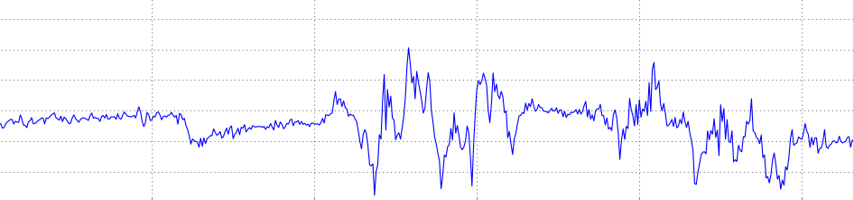
\includegraphics{idling_raw_accelerometer}
    }
    \caption{Single axis accelerometer values while idling}
\end{figure}

\begin{figure}
    \centering
    \resizebox{\textwidth}{!}{
        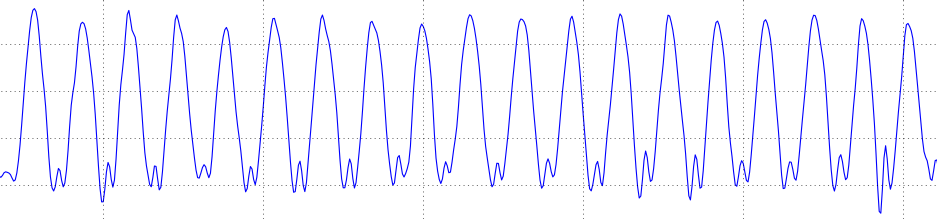
\includegraphics{curl_raw_accelerometer}
    }
    \caption{Single axis accelerometer values while performing curls}
\end{figure}

We have a key intuition, however, to separate exercise from non-exercise, and that is periodicity. Non-exercise tends to be very aperiodic, such as in Figure 3.1, while exercise (especially high-repetition bodybuilder-esque exercise) tends to be very periodic, such as in Figure 3.2. This can be easily exploited then when performing classification. If a certain subset of the signal is highly periodic, it is likely to be an exercise of some kind. However, there is one activity users do in the gym that is both periodic and non-exercise, and that is walking. This necessitates the use of machine learning, as there is no ubiquitous heuristic which can determine both whether a signal is periodic and weather it represents walking versus other exercises. Fortunately, features can easily be extracted and passed into an SVM which accomplishes both of these tasks.

The second issue we face is the \textit{wide variability in form}. We make the assumption that users of this application will have a fundamental understanding of the lifts they perform, although sensor data will inevitably vary depending on physiological features such as height, arm length, and leg length, regardless of how well they perform the repetition. It is possible that a DTW algorithm could allay this, but we choose to simply train our classifiers over a large dataset. By choosing five to ten athletes to provide training data, we can reasonably cover most variations in form. 

Another issue we have is \textit{properly counting}. For an application like a pedometer, counting repetitions becomes almost a trivial task. A heavy low-pass filter can be applied to the signal, and then the number of steps simply becomes the number of peaks. This is due to the relative steadiness with which we walk. Generally speaking, people's gaits do not change much from step to step. A user may walk at a different speed in their house than when they go to class, but on the whole, walking is a cleanly periodic signal. Counting lifting repetitions, however, is a much more difficult task, as the bar speed and repetition rate can change from repetition to repetition, as well as from set to set. A user doing a set of ten repetitions or greater may tire by the end, performing much slower and perhaps even failing a lift. A tracking system must be able to account for this. Additionally, the accelerometer traces of an exercise may not be amenable to simple peak counting, such as in Figure 3.3.

\begin{figure}
    \centering
    \resizebox{\textwidth}{!}{
        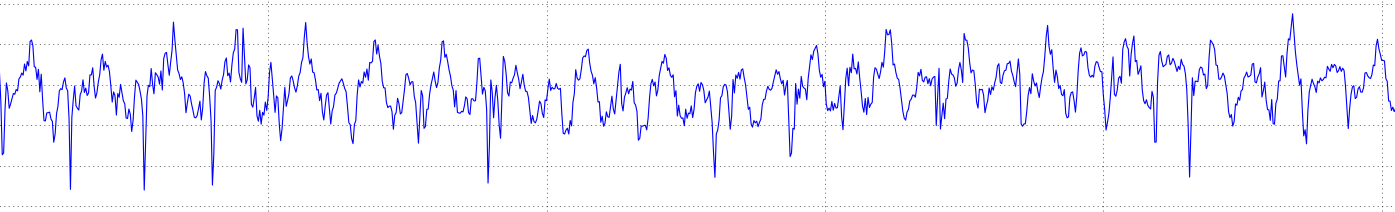
\includegraphics{squat_raw_accelerometer}
    }
    \caption{Single axis accelerometer values while performing squats}
\end{figure}

Finally, we have a problem of \textit{differentiating between similar exercises}. It may be easy for the human eye to differentiate between a Pendlay row and a bench press, but when looking at the movement itself, both simplify down to an explosive upward movement and a controlled downward movement. To this end, we must employ machine learning instead of simple heuristics for lift recognition. 


\section{System Design}

This leads us to our final system design. Our system comprises four primary phases: \textit{preprocessing, segmentation, recognition,} and \textit{counting}. 

First is the \textit{Preprocessing} phase. Android does not guarantee a consistent sampling rate on its sensor readings, thus we first evenly resample the data. Next, we pass the data through a low-pass filter to remove noisy high-frequency components which may not be indicative of the actual lift being performed. This data is then stored for the subsequent three phases.

The \textit{Segmentation} phase is the first phase of intensive computation during which we determine whether or not a lift is being performed. Autocorrelation is computed over a sliding window, then features are extracted and passed into an SVM. The output of this classifier is passed to an accumulator, which acts to smooth any jitter from the classifier. If this phase determines that a lift has been performed, we pass the exercise window to the next phase.

Our \textit{Recognition} phase determines which lift is being performed, given that a lift is actually being performed. Similar feature extraction is done as in the segmentation phase, calculating feature sets over a sliding window. These feature sets are passed to an SVM, and the prediction is stored. As we are using a sliding window, our system makes many predictions for a full exercise window. The final result is determined using a majority voting system.

Once the lift has been successfully recognized, we move to the final phase, \textit{Counting}. Our counting algorithm is essentially a sophisticated method of peak counting. First, we find all local maxima in the signal, discounting peaks if they are too close to one another. Secondly, we use autocorrelation to determine the local periodicity of the signal about a peak and remove peaks that are too close, given the assumption that repetitions may vary over a full signal but will stay relatively consistent from a single repetition to another. Lastly, we use a thresholding heuristic to remove peaks that are too low. The remaining number of peaks is then our final repetition count. 

\section{Equipment}

For testing, we use a first generation Motorola Moto 360 smartwatch running Android Wear v5.0.2. Our smartphone is a Samsung Galaxy S4 running Android v4.4.2. Any combination of smartwatch and smartphone running Android should function with this system, although additional calibration may be needed when working with different smartwatch MEMS sensors. Data collection is performed using the accelerometer and gyroscope on the smartwatch.